\documentclass{aci}

%%%%%%%%%%%%%%%%%%%%%%%%%%%%%%%%%%%%%%%%%%
\usepackage{txfonts}
\usepackage{booktabs}
\usepackage{longtable}
\usepackage{lipsum}
\usepackage{hyperref}
\usepackage{xcolor}
\hypersetup{colorlinks=true}
\usepackage{subcaption}
\usepackage{placeins}
\usepackage{tikz}
\usepackage{makecell}
\usetikzlibrary{automata,positioning,arrows}
\usepackage{caption}
\usepackage{changepage}

%%%%%%%%%%%%%%%%%%%%%%%%%%%%%%%%%%%%%%%%%%
\newcommand{\ep}{\varepsilon}
\newcommand{\eps}[1]{{#1}_{\varepsilon}}

\def\typeofarticle{Research article} 
\def\currentvolume{2} 
\def\currentissue{2}
\def\currentyear{2022} 
\def\currentmonth{} 
\def\ppages{xx--xx} 
\def\DOI{10.3934/aci.2022xxx} 
\def\Received{22 July 2022} 
\def\Revised{31 August 2022}
\def\Accepted{01 September 2022} 
\def\Published{xx 2022}

\numberwithin{equation}{section}
\DeclareMathOperator*{\essinf}{ess\,inf}

\usepackage{array}
\newcolumntype{L}{>{\arraybackslash}m{8cm}}

\hyphenpenalty=10000
\usepackage{cite}
%%%%%%%%%%%%%%%%%%%%%%%%%%%%%%%%%%%%%%%%%%
\begin{document}

\title{Investigation of ant cuticle dataset using image texture
    analysis}

\author{%
    Noah Gardner\affil{1},
    John Paul Hellenbrand\affil{2},
    Anthony Phan\affil{1},
    Haige Zhu\affil{1},
    Zhiling Long\affil{4}, \\
    Min Wang\affil{3},
    Clint Penick\affil{2},
    and Chih-Cheng Hung\affil{1,}\corrauth
}%

% \shortauthors is used in copyright information in the end of the paper
\shortauthors{the Author(s)}

\address{%
    \addr{\affilnum{1}}{Laboratory of Machine Vision and Security Research, %
        College of Computing and Software Engineering, Kennesaw State %
        University, Marietta GA, USA}%
    \addr{\affilnum{2}}{College of Science and Mathematics, Kennesaw State
        University, Kennesaw, GA, USA}%
    \addr{\affilnum{3}}{Department of Mathematics, Kennesaw State University,
        Kennesaw, GA, USA}%
    \addr{\affilnum{4}}{Department of Informatics and Mathematics,
        Mercer University, Atlanta, GA, USA}%
}
\corraddr{Email: chung1@kennesaw.edu.}

\editor{Pasi Fr\"{a}nti}

\begin{abstract}
    Ant cuticle texture presumably provides some type of function, and therefore
    is useful to research for ecological applications and bioinspired designs.
    In this study, we employ statistical image texture analysis and deep machine
    learning methods to classify similar ant species based on morphological
    features. We establish a public database of ant cuticle images for research.
    We provide a comparative study of the performance of image texture
    classification and deep machine learning methods on this ant cuticle dataset.
    Our results show that the deep learning methods give higher accuracy than
    statistical methods in recognizing ant cuticle textures. Our experiments
    also reveal that the deep learning networks designed for image texture
    performs better than the general deep learning networks.
\end{abstract}
\keywords{texture analysis; image processing; classification; machine learning;
    ant cuticle images; ecology}
\maketitle

\section{Introduction}

Insects compose half of biodiversity and rank among the most dominant organisms
in terrestrial ecosystems \cite{sheikh_diverse_2017}. A key factor for the
ecological success of insects is their exoskeleton, also known as cuticle. The
cuticle protects insects from predation, provides structural support, prevents
desiccation, and serves as a canvas for advertising visual and chemical signals
\cite{gullan_insects_2009}. Earlier research has focused on the macrostructures
and internal chemical components that describe the functionality of the
exoskeleton \cite{gunderson_insect_1989}. More recent work is being done to
understand the functional aspects of external cuticle micro sculpturing
\cite{muthukrishnan_insect_2020, watson_diversity_2017}.

Due to the extensive number of insect species, manual exploration of
insect-based information is difficult and often requires expert training.
Therefore, automated entomology has attracted biologists and computer
scientists, and is expected to be a major contribution to the future of
insect-based research~\cite{martineau_survey_2017}. One of the most commonly
used data types for insect analysis is image data. To develop an image-based
system for insect analysis, we can utilize existing work in general
image analysis methods.

We study ants (\textit{Formicidae}) as they display an extreme diversity of
cuticle micro sculpturing across all subfamilies. Microsculpture ranges from
parallel longitudinal ridges to deep oval impressions to erratic protuberances.
Microsculpture has arisen convergently and independently throughout ant's
evolutionary history, which suggests  that these are complex traits undergoing
selection. Cuticle microsculpture on ants may help increase strength and
rigidness, resist abrasion, increase internal and external surface area, resist
microbial growth, and cultivate beneficial anti-biotic producing bacteria
\cite{johnson_effect_2011, bruckner_relationship_2017, currie_coevolved_2006}.
These specific functions may be associated with certain sculpturing types. To
analyze those functions, we first segment the image and group similar textures
for further analysis.

There is a large variety of ant species and most species are diverse in terms of
size, shape, behaviors, and cuticle textures \cite{harris_glossary_1979}. Based
on our initial observation of the cuticle sculpturing in ants, it appears that
some type of textural structures can be identified in images. Therefore, it is
worthwhile to explore image texture analysis for further knowledge discovery.
Image texture analysis has been used in image processing for many decades
\cite{hung_image_2019}. Due to the diversity of images on scales, smoothness,
coarseness, microtexture, and macrotexture occurring in images, it is a
difficult problem. With a rapid development of deep machine learning, deep
neural networks have been frequently used in image texture analysis in other
fields \cite{sun_robust_2014,liu_bow_2019,liu_pestnet_2019}.

Our contribution is to establish an ant image dataset which can be used to
explore the categorization of different ant cuticle textures using image texture
analysis methods. We document how the dataset of ant cuticle images is
established. Our experiment shows that the deep learning networks designed for
image texture analysis give a better accuracy than classical K-views clustering.

This paper is organized as below:  Section 2 reviews the microsculpturing
identification in ants, and image texture analysis and insect classification.
Section 3 describes the dataset preparation and image texture analysis methods
used in our experiments. Section 4 gives the experimental setup and methods
used. Section 5 shares visualization of both raw and processed images, and
analysis of experimental results. The conclusion then follows.

\section{Related work}

In this section we review related work on microsculpturing identification, image
texture analysis, and insect classification.

\subsection{Microsculpturing identification}

Because ants lack bold coloration and complex wing venation patterns used to
identify other insect species, microsculpturing has taken a prominent role in
ant identification. To aid in species identification, ant taxonomists have
developed nearly 100 terms to describe  fine differences in microsculpturing
patterns \cite{harris_glossary_1979, bolton_identification_1994}. Despite the
prominent role of microsculpturing in ant identification, however, almost
nothing is known about how these patterns evolved or their function. Similar
microsculpturing patterns in other organisms have been found to reduce abrasion,
increase stiffness, and perform as structural antibiotics
\cite{zhiwu_erosion_2012, han_efficient_2015, rees_form_1975,
    chung_impact_2007,hasan_selective_2013}. Developing a better understanding of
the function of microsculpturing in ants could provide insight into their
evolution and biology as well as lead to the development of bio-inspired
technologies \cite{penick_comparative_2022}.

One challenge for functional investigations of cuticle microsculpturing is the
complexity of terms used to describe these patterns. Complex terminology may be
useful for describing fine differences between closely related species, but
broader comparisons require a simplified classification scheme. We recently
developed a classification system for microsculpturing that consists of only
five categories: smooth, striate, punctate, reticulate, and tuberous
\cite{hellenbrand_ant_2022}. We used these categories to classify 11,722 ant
species, and found that the earliest ants were smooth and that cuticle
microsculpturing independently evolved later in multiple lineages
\cite{hellenbrand_ant_2022}. A simple classification scheme divides ants into
two categories: smooth and rough. Because microsculptuing has evolved numerous
times in ants, this binary classification scheme is sufficient.

The next challenge is to find out how to apply these schemes to large numbers of
species. Insect researchers have access to millions of images available through
digital museum collections \cite{beaman_mass_2012}. Going through these digital
collections manually is not feasible for large projects. There are over 14,000
described species of ants, and each species has multiple worker and reproductive
castes that may vary in their microsculpturing patterns. Even within an
individual ant, microsculpturing typically varies among and within body
segments. Machine learning offers a solution to this problem through developing
tools that automate trait classification. Automated approaches would allow
researchers to leverage existing image repositories to extract large trait
datasets that can then be used to detect evolutionary patterns.


\subsection{Image texture analysis}

Pattern recognition methods have been developed for textural images based on the
spatial relationship of gray levels of pixels encoded in the texture
\cite{haralick_image_1985,hung_image_2019}. Those methods extract texture
features and the classification and segmentation methods are used for the
interpretation either using the supervised or unsupervised approaches
\cite{fukunaga_introduction_2013}. The interpretation method is usually modified
from the traditional pattern recognition methods. For example, the gray-level
co-occurrence matrix (GLCM) and local binary patterns (LBP) are two common
methods for extracting features \cite{haralick_textural_1973, goos_gray_2000}.

Classical image texture analysis methods can be grouped into four categories:
statistical, structural, model-based, and transform-based methods
\cite{bharati_image_2004}. The statistical method is often used for image
classification after feature extraction. Markov random field models have also
been used for textural image interpretation \cite{hassner_use_1981,
    cross_markov_1983}. Transform-based methods use some functions to decompose an
image texture into a set of basic feature images. Gabor filters and wavelet
expansions are two of the widely used approaches \cite{bovik_multichannel_1990}.

Liu et al. gave a comprehensive survey on textural characterization in which
they call this feature extraction as texture representation \cite{liu_bow_2019}.
Their survey on bag of words and convolutional neural networks (CNNs)
\cite{krizhevsky_imagenet_2017} provides information on spatial relationship
concepts. The K-views was developed for taking the spatial information in the
clustering approach \cite{hung_image_2019}.

\subsection{Deep learning for texture analysis}

In the past decade, deep learning using CNNs has emerged as the mainstream
technology for image analysis. Following this trend, various related network
architectures have been designed to specifically characterize textural images.
Among these, the Fisher-vector CNN descriptor (FV-CNN) proposed by Cimpoi et al.
\cite{cimpoi_deep_2015} is widely accepted as one of the pioneering works. It
applies Fisher-vector pooling to deep features obtained via a CNN pre-trained
using the ImageNet \cite{krizhevsky_imagenet_2017} to obtain encoded features
for texture classification. FV-CNN is capable of achieving higher classification
accuracy comparing to traditional hand-crafted texture features. However,
CNN-based deep learning is only used in its feature extraction module. Its
encoding and classification modules still use traditional learning methods, thus
not supporting an \textit{end-to-end} deep learning. In the context of texture
image classification, an end-to-end deep learning model refers to a neural
network architecture which consists of all the modules (feature extraction,
encoding and classification) between the initial input data and the final output
classification result, with all the modules being trained simultaneously.

To achieve an end-to-end learning, Zhang et al. \cite{zhang_deep_2017} proposed
the deep texture encoding network (DeepTEN), in which a novel texture encoding
layer is added to a standard CNN architecture. Then, Xue et al.
\cite{xue_deep_2018} constructed the deep encoding pooling network which
improves over DeepTEN by integrating local spatial characteristics into the
texture representation. Based on these two methods, Hu et al. \cite{hu_multi_2019}
further developed the multi-level texture encoding and representation (MuLTER)
network, which embeds a learnable encoding module at each convolutional layer so
that encoding is performed for both low-level and high-level features, yielding
a multi-level texture representation.

Other network architectures for end-to-end texture learning are also available.
For example, in the deep multiple-attribute-perceived network (MAP-Net)
\cite{zhai_deep_2019}, multiple perceptual attributes are progressively learned
in a mutually reinforced manner through multiple branches. In the deep
structure-revealed network (DSR-Net) \cite{zhai_deep_2020}, inherent structural
representation for a texture pattern is obtained by employing a primitive
capturing module to learn spatial primitives and a dependency learning module to
capture the dependency among the primitives. In \cite{mao_deep_2021}, a residual
pooling layer consisting of a residual encoding module and an aggregation module
is used to generate discriminative features of low dimensions. In
\cite{peeples_histogram_2021}, a histogram layer is designed to compute local
spatial distribution of CNN features. In \cite{chen_deep_2021}, an innovative
aggregation module is presented to exploit statistical self-similarity across
layers. All these architectures customize the standard CNN structure to
accomplish the characterization of certain spatial, visual, and statistical
traits unique to textural images.

Compared with the traditional method in which a kernel must be designed by an
engineer for extracting features, the deep learning networks can automatically
extract the features through the training. In addition, the deep learning
networks can 6achieve the higher accuracy than that of the classical approaches,
although the deep networks require much more data for training.

\subsection{Classification of insects}

Proposed insect classification methods seek to classify insects at different
hierarchical levels, such as species, genus, family, and order. Additionally,
some methods may classify insects at a combination of different hierarchical
levels. Insect classification methods can be applied to a variety of fields. In
agriculture, insect classification methods can be used to identify the presence
of pest insects in crops, which can inform crop managers in their choice of
pesticides and help prevent crop loss \cite{liu_pestnet_2019,
    kasinathan_machine_2021}.

Feng et al. \cite{feng_automated_2013} apply an automated system to classify
moth images based on semantic related visual attributes, which are defined as a
pattern on the moth wings. Feng et al. \cite{feng_automated_2013} use a custom
texture descriptor based on the combination of GLCM and \textit{scale-invariant
    feature transform} (SIFT) features \cite{gotlieb_texture_1990,
    lowe_distinctive_2004}. The method is used to classify 50 different moth species
across 8 families \cite{feng_automated_2013}. Their results
\cite{feng_automated_2013} suggest that traditional feature extraction
techniques for the semantic visual attributes of the moth wings are sufficient
for training a classifier to classify an image between 10 randomly selected moth
species. Marques et al. \cite{marques_ant_2018} propose an ensemble-based method
to classify a large number of ant genera. They use ant head, profile, and dorsal
images sourced from AntWeb in order to classify 44,806 specimens with at least
one picture into 57 genera. Although the images used in their work are also from
AntWeb, our goal is the classification of the ant cuticle micro sculpturing into
broad groups based solely on the ant head images.

Urteaga et al. \cite{urteaga_scorpions_2016} use machine learning methods in
order to classify images between two different scorpion species:
\textit{Centruroides limpidus} and \textit{Centruroides noxius}. After applying
background distinction based on dynamic color threshold, they extract features
from the separated scorpion image such as aspect ratio, rectangularity, and
compactness. They apply three different models to classify the image as one of
the species: artificial neural network, regression tree, and random forest
classifiers \cite{urteaga_scorpions_2016}. Their results show that after
background removal, characteristics from the entire body of the scorpion can be
used to create a binary classifier that can classify the image as one of the two
species.

Lim et al. \cite{lim_performance_2017} apply a CNN-based algorithm for insect
classification. Lim et al. \cite{lim_performance_2017} classify a subset of
insect species and families based on the classes available in the ImageNet
dataset. ImageNet is a widely used dataset of images labeled by experts with
millions of images and thousands of categories~\cite{deng_imagenet_2009}. In the
ImageNet dataset, there are some categories that specify the class of the insect
on a species level, e.g. \textit{monarch butterfly} and \textit{ringlet
    butterfly} as well as some categories that specify the class of the insect on a
family level, e.g. \textit{ant}, \textit{fly}, and \textit{bee}
\cite{deng_imagenet_2009}. Lim et al. \cite{lim_performance_2017} use a modified
AlexNet architecture and experiment with different numbers of kernels and their
effect the performance of the model. Glick et al. \cite{glick_insect_2016}
employ a similar approach by classifying 277 insect classes from ImageNet using
a hierarchical convolutional neural network. The results from Lim et al.
\cite{lim_performance_2017} and Glick et al. \cite{glick_insect_2016} suggest
that a CNN is capable of differentiating between different hierarchical classes
of insects.

\section{Ant cuticle image dataset}

% \subsection{Dataset preparation} % preparation generation

In this section, we describe the creation of the custom dataset used in this
research. We use ant head images from AntWeb \cite{perrichot_antweb_2012} and
define two categories for them based on the appearance of the cuticle texture:
\textit{rough} and \textit{smooth}. The original AntWeb dataset was extended
with these categories for each applicable ant specimen. The extended dataset is
used for classifying the cuticle micro sculpturing into the broad groups. Due to
the large number of ant species, it is quite difficult to obtain lab-quality
specimen photos. For each species used, there exists only one ant head image. We
also refer to these ant head images, which describe the pose of the ant, as ant
cuticule images, due to the clear cuticle texture present on the head. Some
randomly selected images from each category are shown in Figures
\ref{fig:smooth-cuticle-texture} and \ref{fig:rough-cuticle-texture}.

To begin, a master spreadsheet was created with the 2,499 different ant species
to be identified for the primary dataset. The team was trained to identify
cuticle sculpturing through a process which consisted of one 45-minute
introductory lesson explaining the project and texture categories. Then, the
team was given a training set of photos to identify from the genus
\textit{Polyrhachis}. The sculpture identification protocol describes the two
primary categories: rough and smooth.

\begin{figure}[h]
    \centering
    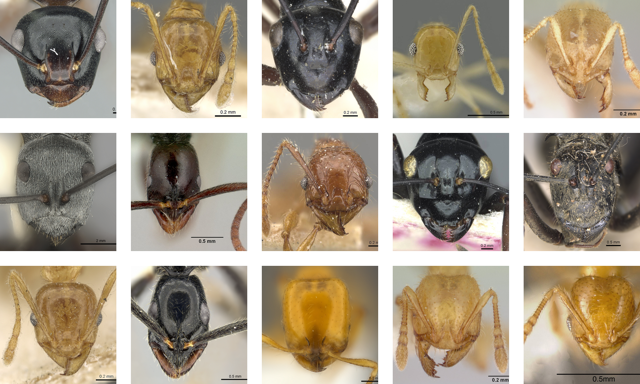
\includegraphics[width=0.7\textwidth]{assets/images/smooth_full_collage.png}
    \caption{Examples of smooth cuticle texture ant images in the dataset after
        center cropping, from AntWeb \cite{perrichot_antweb_2012}.}
    \label{fig:smooth-cuticle-texture}
\end{figure}

\begin{figure}[h]
    \centering
    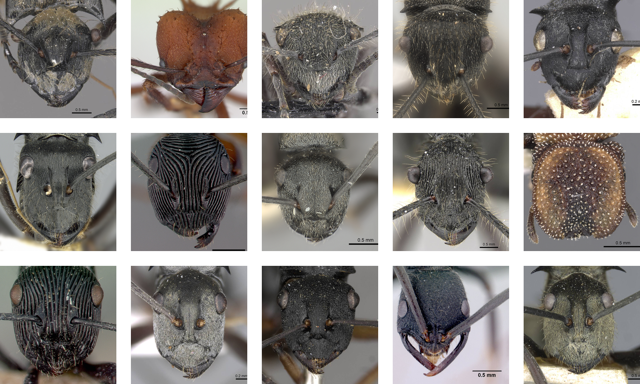
\includegraphics[width=0.7\textwidth]{assets/images/rough_full_collage.png}
    \caption{Examples of rough cuticle texture ant images in the dataset after
        center cropping, from AntWeb \cite{perrichot_antweb_2012}.}
    \label{fig:rough-cuticle-texture}
\end{figure}

Initially, the sculpture identification protocol had five subcategories of
cuticle texture: smooth, punctate, striate, reticulate, and tuberous. For
simplicity, we worked only with the two main categories, and the other four
categories were combined to the single rough category. The training set
identifications were reviewed together as a group by the assistants. Once
training was complete, assistants were assigned the same genera of ants to
identify independently each week. A weekly meeting was held to discuss
identifications and assign new ones. These identifications were collected in the
master spreadsheet and the identifications were assigned to individual ant
species on a majority basis.

To collect the images from AntWeb\footnote{\url{https://www.antweb.org/}}, the
assistants followed the taxonomy information available in the master spreadsheet
to the appropriate AntWeb page. In many cases, there are multiple ant head
images of the same species, and occasionally there are multiple image resolution
available from a single image. To simplify the data collection process, the
assistants were instructed to download the first ant head image of the species
being identified in the highest resolution possible. Each image was named with
an identifier that corresponds with the row number in the master spreadsheet.
The same ant head images that were downloaded in the data collection phase were
the same ones used in the sculpture identification protocol. Ant species which
did not have any images of the head were excluded from the dataset.
Additionally, ant species which only had a head image of a queen ant were
excluded from the dataset.

Ant specimen images in AntWeb \cite{perrichot_antweb_2012} are created by
different photographers and therefore have different attributes, such as
environment, resolution, and lighting. In the ant head images, the ant head is
in the center of the image and the body is pointing away from the camera. The
focus of the ant head image is centered on the head, with the background and
image artifacts from the ant body typically blurred. In most ant head images,
there is a bar which indicates the scale of the image due to the variety in the
sizes of different ant species. In a few ant head images, there exists some text
denoting the specimen identifier and other information. In terms of texture,
some ant specimens are very old, so their head images have other abnormalities
such as cracks in the cuticle and the presence of dust.

The completed dataset\footnote{The dataset is available on GitHub
    \url{https://github.com/ngngardner/cuticulus}} contains 2,499 images as a
4-dimensional array with shape of (samples, rows, columns, channels), of
which there are 3 channels extracted from the RGB images. 1072 samples of
rough textured ant cuticle textures comprise 43\% of the dataset. The
remaining 1427 samples of smooth textured ant cuticle textures comprise 57\%
of the dataset. Due to the variety of the ant head image attributes, we
apply simple preprocessing before the images are used in our model. We want
the images to have a uniform size for simplicity in our classification
process. Since the ant head images are typically centered in the image, we
apply a center crop to each image to create a square image of the same size.
Once the image is square, we resize each image to a fixed size of 256 $\times$ 256
pixels. We leave other discrepancies in the images untouched. A summary of
the resulting dataset is shared in Table \ref{tab:dataset-summary}.

\begin{table}[h]
    \centering
    \caption{Summary of the dataset.}
    \begin{tabular}{|l|c|}
        \toprule
        Total images  & 2499             \\
        Rough images  & 1072             \\
        Smooth images & 1427             \\
        Image size    & 256 $\times$ 256 \\
        \bottomrule
    \end{tabular}
    \label{tab:dataset-summary}
\end{table}

\section{Methods tested}

% \subsection{Classical texture analysis methods}

The K-means algorithm is one of widely used clustering algorithms in the pattern
recognition \cite{lloyd_least_1982}. It is a single pixel based classification
algorithm for images. Based on the concept of K-means, K-views was developed,
which uses characteristic views for image texture representation
\cite{hung_use_2002}. The K-views algorithm is suitable for classifying image
textures that have basic local patterns repeated in a periodic manner. In
contrast to the K-means, K-views looks at the neighboring pixels for providing
the spatial relationship for classification.

For the feasibility study in these ant image datasets, we tested the statistical
clustering methods and deep learning methods separately. Both K-means and
K-views were used for statistical clustering methods. The experiments may
indicate how well the statistical approach and deep learning networks will do in
this type of textural images. A pre-processing step of the dataset for the
statistical clustering methods is shown below. This pre-processing will
highlight some of characteristic features in textures, such as edge-like in the
image. This step is very useful in feeding the datasets to the K-views
algorithms. In order to classify an image with K-views or K-means in which we
count the number of pixels assigned to each cluster. A brief procedure for
K-views experiments is given below for training and classification.
\begin{description}
    \item[Step 1:] Pre-processing the dataset: apply the Gabor filter to
          transform the gray-scale ant image into four Gabor-filtered channels,
          subtract the gray-scale image from each channel, and take the absolute
          value of the resulting images. The theta θ parameters in the Gabor
          filters used are multiples of π/4 radians starting from 0 to π
          radians. The Gabor filter lambda λ parameter is equal to π.

    \item[Step 2:] Initialize k = 3 clusters; one for background, and the other
          two as rough and smooth.

    \item[Step 3:] Extract patches for each cluster for the clustering.

    \item[Step 4:] Calculate the mean of each cluster once the training
          converges.

    \item[Step 5:] Use the mean of the cluster for the classification. To
          determine if an image is rough or smooth, we choose the cluster with
          the majority number of pixels. The number of pixels assigned to the
          background cluster are ignored for classification.
\end{description}

\noindent Steps 2 to 4 are for training and step 5 is for the classification.
For the K-means experiments, it will be the same as the K-views except no
patches are used.
\newline
% \subsection{Deep learning models used for the experiments}

The first deep learning model used in our experiment is \textit{visual geometry
    group} (VGG), a convolutional neural network that takes advantage of very
small convolutional filters in a deep network architecture
\cite{simonyan_very_2015}. We compare four architectures of VGG11, VGG13,
VGG16, and VGG19. The primary difference between the architectures is the
number of layers in each model. The second deep learning model used in our
experiments is \textit{residual network} (ResNet), a deep network
architecture that includes shortcut connections between layers (residual
connections) \cite{he_deep_2015}. We compare three architectures of
ResNet18, ResNet50, and ResNet101. Again, the primary difference between the
architectures is the number of layers in each model.

For the initial ResNet models, we have two versions: randomized and pretrained.
The randomized version is the same architecture, but the weights are randomly
initialized. The pretrained version has weights from training on the CIFAR
dataset, an image dataset with 1000 classes. Since the pretrained weights are
readily available, we also evaluate a fine-tuned model. For VGG, we only use the
randomized version. The base VGG architecture also has an output layer of size
1000. Since we are working with a binary classification problem, we modify the
architecture for all models to have an output layer of size 2. Each model is
trained over 100 epochs, using stochastic gradient descent with momentum. The
batch size is set to 16 images. We apply a learning rate of 0.001 and momentum
parameter of 0.9.

% \subsection{Deep texture analysis method used for the experiments}

In addition to the classical texture analysis methods and the deep learning
models for general image analysis, we also examine deep learning analysis
methods specifically designed for textural images. For this examination, we
adopt the deep residual pooling (DRP) network \cite{mao_deep_2021}. The DRP
framework consists of a unique residual pooling layer, which is formed by a
residual encoding module followed by an aggregation module. The residual
encoding module extracts relevant spatial information, while the aggregation
module performs averaging to obtain orderless low-dimension features for
classification.

According to \cite{mao_deep_2021}, the DRP network can be used either with a
single residual pooling layer, applied right before the classifier layer, or
with multiple residual pooling layers, applied to the output of multiple
convolutional layers before feeding the combined pooling results into the
classifier layer. Additionally, an auxiliary classifier layer may also be used.
In our experiments, we follow the same strategy. For each scenario, we conduct
two experiments. One experiment employs weights that are randomly initialized,
and the other uses weights that are fine tuned over those from a pretrained
model.

To handle the imbalance of the dataset, we apply undersampling for each class
for the training dataset \cite{tiittanen_novel_2022}. By using random stratified
sampling, we construct a training set with 800 images per class. The remaining
images are randomly split between test and validation, which turns out to
roughly a 60\%/20\%/20\% train, test, and validation data split. With 272 rough
samples and 627 smooth samples left over after the stratified split, the test
dataset has roughly 136 rough samples and 313 smooth samples. Since these
leftover samples are split with code by 50\% there will be some rounding
variance and therefore the test dataset built at run-time will not always have
exactly the same number of samples.

% \subsection{Evaluation}

We evaluate the performance of the models using accuracy, precision, F1 score
and Matthew's correlation coefficient (MCC) \cite{chicco_matthews_2021}. We also
apply Grad-CAM with manual inspection to visualize the activation weights for
classified images to show which features lead to the classification result.
Finally, we apply t-SNE to visualize the separation learned for the model to
further analyze the classifications made by the model.

\section{Results}

% \subsection{Environment}

Experiments were run on an Ubuntu 18.04 LTS Lambda Labs GPU server. The server
contained 8 NVIDIA GeForce RTX 2080 Ti graphics cards with 12GB of memory each.
The server used an Intel Xeon Silver 4116 with 48 total threads and maximum
frequency of 3.000 GHz, and has 256GB of RAM. K-means algorithm comes from the
scikit-learn\footnote{\url{https://scikit-learn.org/}} library. The K-views
implementation was based on the K-means implementation from scikit-learn. VGG
and ResNet models come from the
torchvision\footnote{\url{https://pytorch.org/vision}} library. DRP model code
was tweaked from the original author's uploaded code on
GitHub\footnote{\url{https://github.com/maoshangbo/DRP-Texture-Recognition}}.

The results show that the fine-tuned ResNet models outperform the VGG and
randomly initialized ResNet models on the task of ant head image classification.
The DRP models perform better than the the general deep learning models VGG and
ResNet on the task of ant head image classification. The fine-tuned DRP
single-layer model with auxiliary classifier performed the best with an average
F1 score of 0.92. We further analyze the separation learned by both ResNet101
models in the following section.

% \subsection{Experimental results}

We share the results on each algorithm specified in Section 4. Both the K-means
and K-views algorithms are unsupervised. All of the deep learning methods used
are supervised. The results are shown in Table \ref{tab:results}. It should be
noted that due to the class imbalance in the dataset, the F1 score is the
preferable metric to the accuracy.
% Therefore, the results have been sorted by F1 score in descending order.

\begin{table}[h]
    \centering
    \caption{Experimental results of different algorithms}
    \small
    \begin{tabular}{lcccc}
    \toprule
    Model                                   & Accuracy & Precision & Recall & F1   \\
    \midrule
    K-means                                 & 0.47     & 0.07      & 0.35   & 0.11 \\
    K-views (15 $\times$ 15)                & 0.56     & 0.58      & 0.56   & 0.57 \\
    K-views (17 $\times$ 17)                & 0.62     & 0.79      & 0.59   & 0.68 \\
    K-views (19 $\times$ 19)                & 0.62     & 0.80      & 0.59   & 0.68 \\
    K-views (25 $\times$ 25)                & 0.52     & 0.71      & 0.51   & 0.59 \\
    \hline
    ResNet18                                & 0.80     & 0.72      & 0.67   & 0.69 \\
    ResNet18 (fine-tuned)                   & 0.88     & 0.87      & 0.77   & 0.82 \\
    ResNet50                                & 0.78     & 0.59      & 0.67   & 0.62 \\
    ResNet50 (fine-tuned)                   & 0.87     & 0.83      & 0.78   & 0.80 \\
    ResNet101                               & 0.77     & 0.63      & 0.62   & 0.62 \\
    ResNet101 (fine-tuned)                  & 0.89     & 0.87      & 0.78   & 0.82 \\
    \hline
    VGG11                                   & 0.80     & 0.73      & 0.66   & 0.69 \\
    VGG13                                   & 0.82     & 0.69      & 0.71   & 0.69 \\
    VGG16                                   & 0.80     & 0.65      & 0.67   & 0.65 \\
    VGG19                                   & 0.81     & 0.67      & 0.68   & 0.64 \\
    \hline
    DRP Multi-layer                         & 0.87     & 0.89      & 0.92   & 0.91 \\
    DRP Multi-layer (fine-tuned)            & 0.88     & 0.89      & 0.93   & 0.91 \\
    DRP Single-layer                        & 0.88     & 0.90      & 0.94   & 0.92 \\
    DRP Single-layer (fine-tuned)           & 0.88     & 0.90      & 0.93   & 0.91 \\
    DRP Single-layer Auxiliary              & 0.87     & 0.89      & 0.92   & 0.90 \\
    DRP Single-layer Auxiliary (fine-tuned) & 0.89     & 0.90      & 0.94   & 0.92 \\
    \bottomrule
\end{tabular}

    \label{tab:results}
\end{table}

%\FloatBarrier



% \colorbox{green}{(TODO: DRP is best performing model, it should be included in
%     visualization.)}

% \subsection{Clustering segmentation}

% \subsection{t-SNE Visualization}

\begin{figure}[h!]
    \centering
    \begin{subfigure}{.45\textwidth}
        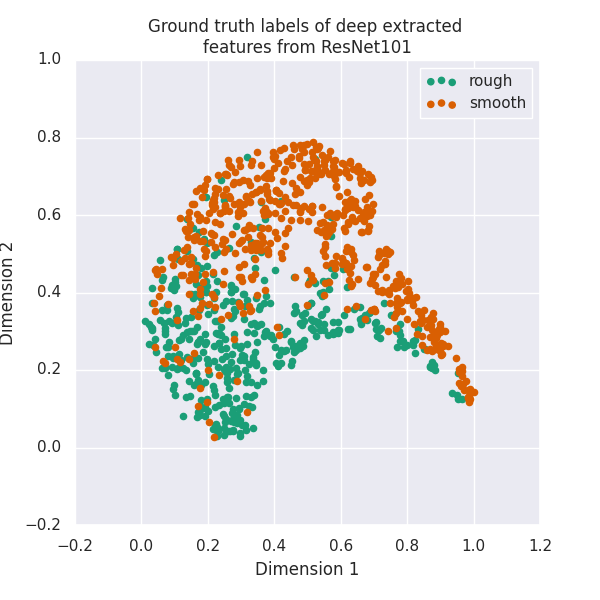
\includegraphics[width=1\linewidth]{thesis_assets/plots/resnet101_gt_tsne.png}
        % \caption{Ground truth labels}
    \end{subfigure}
    \begin{subfigure}{.45\textwidth}
        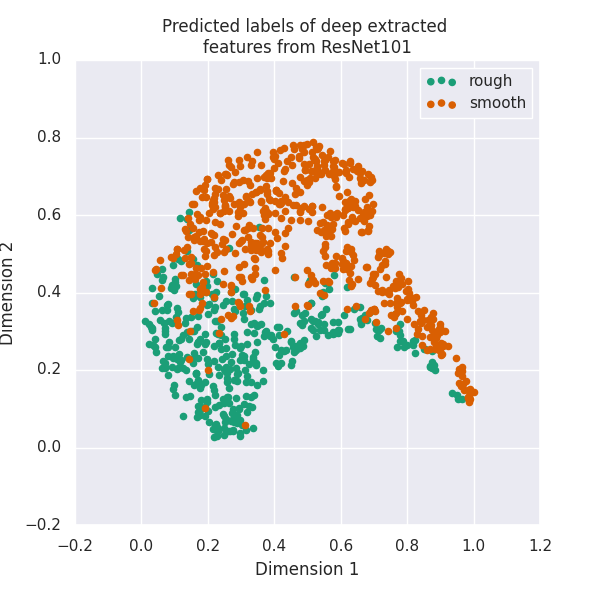
\includegraphics[width=1\linewidth]{thesis_assets/plots/resnet101_pred_tsne.png}
        % \caption{Predicted labels}
    \end{subfigure}
    \caption{t-SNE visualization of the embeddings of the second to last layer
        of the randomly initialized ResNet101 model trained on dataset.}
    \label{fig:resnet101_tsne}
\end{figure}

In this section, we provide visualization of the fine-tuned ResNet101 model and
the randomly initialized ResNet101 model using t-SNE dimensionality reduction.
To visualize the deep extracted features, we modify each model to obtain the
embeddings of the second to last layer. We plot side-by-side the ground truth
and predicted labels for each model. Figure \ref{fig:resnet101_tsne} shows the
results of the trained randomly initialized model and Figure
\ref{fig:fresnet101_tsne} shows the results of the fine-tuned model. Based on
the visual results of the t-SNE visualization, we can see that the fine-tuned
model learned a stronger separation of the two classes, which reinforces the
results that the fine-tuned model received a higher average accuracy.

\begin{figure}[h!]
    \centering
    \begin{subfigure}{.45\textwidth}
        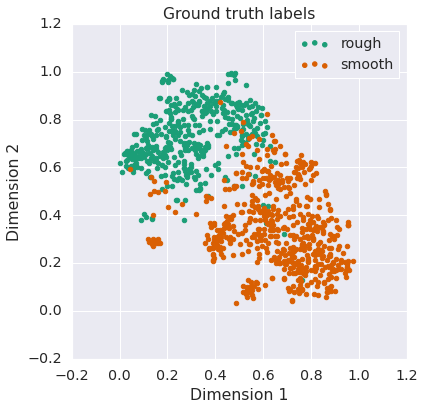
\includegraphics[width=1\linewidth]{thesis_assets/plots/fresnet101_gt_tsne.png}
        % \caption{Ground truth labels}
    \end{subfigure}
    \begin{subfigure}{.45\textwidth}
        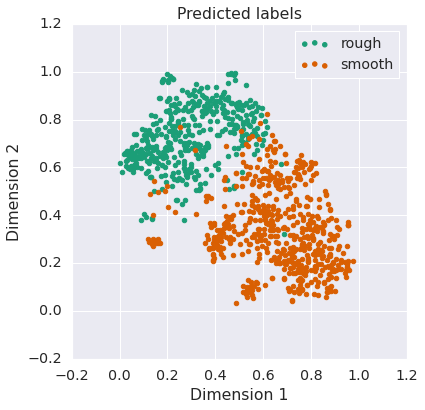
\includegraphics[width=1\linewidth]{thesis_assets/plots/fresnet101_pred_tsne.png}
        % \caption{Predicted labels}
    \end{subfigure}
    \caption{t-SNE visualization of the embeddings of the second to last layer
        of the fine-tuned ResNet101 model trained on dataset.}
    \label{fig:fresnet101_tsne}
\end{figure}


% \subsection{GradCAM visualization}

Next, we provide some visual analysis of some correctly and incorrectly
classified images using GradCAM. In the expected case, the features that are
used to compute the classification are the same as the features used by the
assistants in the sculpture identification process. In general, the features
used by the assistants are the textures of the cuticle on the ant head. In the
non-expected case, the features used to compute the classification are not from
the head, for example, from the background, extraneous text, or the body of the
ant. We used randomly selected images from the dataset and the fine-tuned
ResNet101 model to perform the analysis. We show the GradCAM results in Figures
\ref{fig:correct_images} and \ref{fig:incorrect_images}. The left image shows
the preprocessed image input to the model. The right image shows the GradCAM
output based on the classification. Four specimens were selected randomly from
each category and subcategory.

Correctly classified images which use the expected features show the ideal
performance of the model. Incorrectly classified images which use the expected
features should be further analyzed. In essence, the model in this situation
knows \textit{where} to look, but not \textit{what} to look for. In Figure
\ref{fig:incorrect_images}, there are results where the features activated are
mostly in the correct location on the ant head, and the rough texture is clearly
visible, yet the model predicts the incorrect class \textit{smooth}. Similarly
in Figure \ref{fig:incorrect_images}, there are results where the features
activated are also mostly in the correct location, yet the model predicts the
incorrect class \textit{smooth}. In this case, it may be due to the pose of the
ant being slightly different from the average pose. In the incorrectly
classified images with non-expected features, analysis shows that the model is
unable to find \textit{where} to look, and obtains feature information from
other parts of the ant or the background. Cases where the image was correctly
classified using the non-expected features can basically be seen as noise. In
order to further analyze this class, we should introduce some parameter such as
model confidence to examine further.

\newcommand{\subwidth}{0.35\textwidth}
\begin{figure}
    \centering
    \begin{subfigure}{\subwidth}
        \caption*{Smooth texture}
        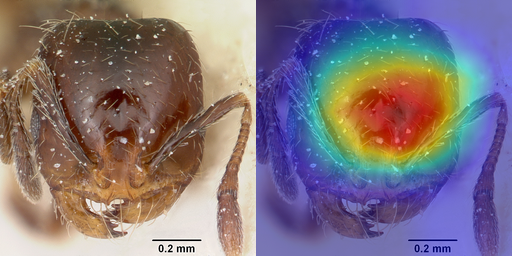
\includegraphics[width=1\linewidth]{thesis_assets/gradcam/correct_ideal/518.png}
        \label{fig:correct_ideal_518}
    \end{subfigure}
    \begin{subfigure}{\subwidth}
        \caption*{Smooth texture}
        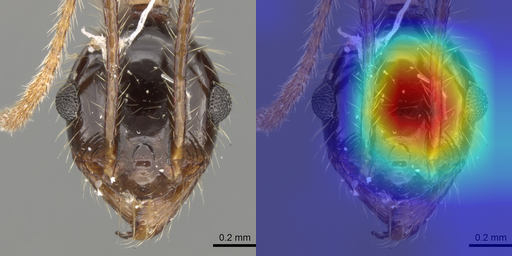
\includegraphics[width=1\linewidth]{thesis_assets/gradcam/correct_ideal/808.png}
        \label{fig:correct_ideal_808}
    \end{subfigure}
    \begin{subfigure}{\subwidth}
        \caption*{Rough texture}
        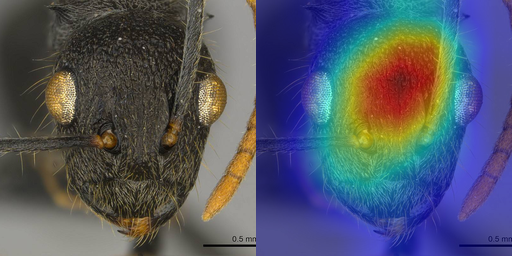
\includegraphics[width=1\linewidth]{thesis_assets/gradcam/correct_ideal/842.png}
        \label{fig:correct_ideal_842}
    \end{subfigure}
    \begin{subfigure}{\subwidth}
        \caption*{Rough texture}
        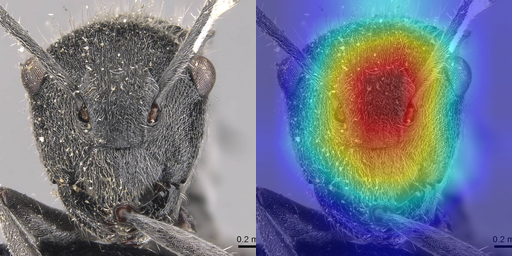
\includegraphics[width=1\linewidth]{thesis_assets/gradcam/correct_ideal/1091.png}
        \label{fig:correct_ideal_1091}
    \end{subfigure}
    \begin{subfigure}{\subwidth}
        \caption*{Rough texture}
        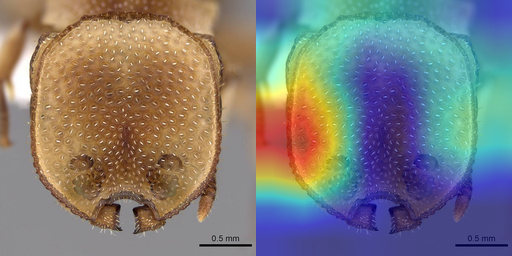
\includegraphics[width=1\linewidth]{thesis_assets/gradcam/correct_nonideal/346.png}
        \label{fig:correct_nonideal_346}
    \end{subfigure}
    \begin{subfigure}{\subwidth}
        \caption*{Rough texture}
        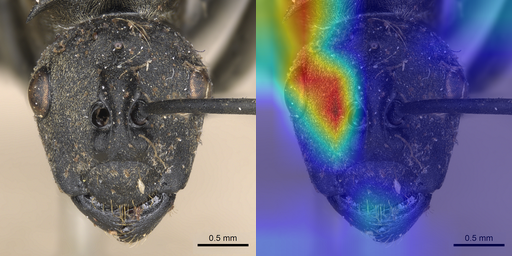
\includegraphics[width=1\linewidth]{thesis_assets/gradcam/correct_nonideal/1554.png}
        \label{fig:correct_nonideal_1554}
    \end{subfigure}
    \begin{subfigure}{\subwidth}
        \caption*{Rough texture}
        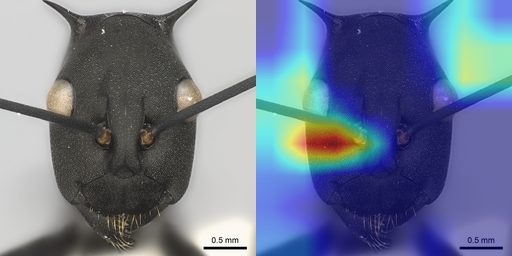
\includegraphics[width=1\linewidth]{thesis_assets/gradcam/correct_nonideal/1694.png}
        \label{fig:correct_nonideal_1694}
    \end{subfigure}
    \begin{subfigure}{\subwidth}
        \caption*{Smooth texture}
        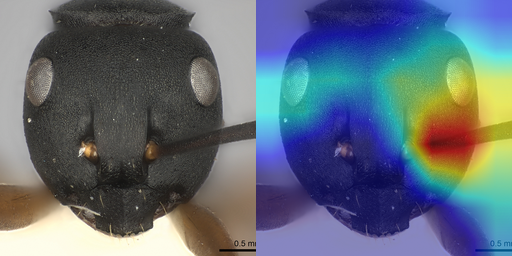
\includegraphics[width=1\linewidth]{thesis_assets/gradcam/correct_nonideal/388.png}
        \label{fig:correct_nonideal_388}
    \end{subfigure}
    \caption{GradCAM visualization for correctly classified images from
        fine-tuned ResNet101. The red sections of the heatmap show which features
        had higher activation for the classication.}
    \label{fig:correct_images}
\end{figure}

\begin{figure}
    \centering
    \begin{subfigure}{\subwidth}
        \caption*{Rough texture}
        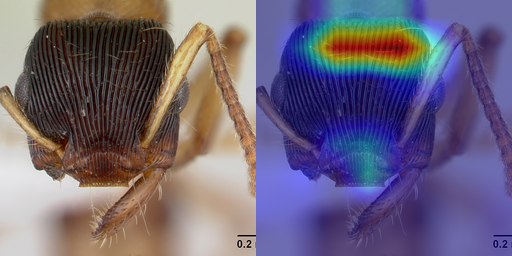
\includegraphics[width=1\linewidth]{thesis_assets/gradcam/incorrect_ideal/84.png}
        \label{fig:incorrect_ideal_84}
    \end{subfigure}
    \begin{subfigure}{\subwidth}
        \caption*{Smooth texture}
        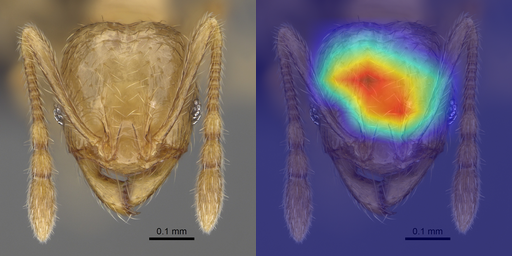
\includegraphics[width=1\linewidth]{thesis_assets/gradcam/incorrect_ideal/86.png}
        \label{fig:incorrect_ideal_86}
    \end{subfigure}
    \begin{subfigure}{\subwidth}
        \caption*{Smooth texture}
        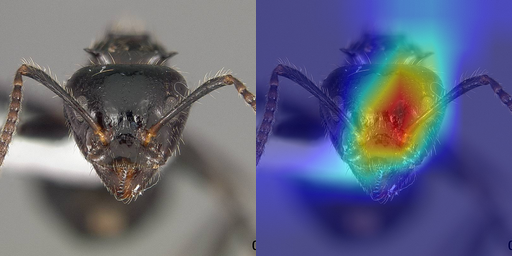
\includegraphics[width=1\linewidth]{thesis_assets/gradcam/incorrect_ideal/177.png}
        \label{fig:incorrect_ideal_177}
    \end{subfigure}
    \begin{subfigure}{\subwidth}
        \caption*{Smooth texture}
        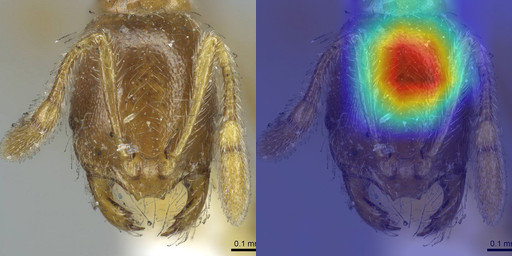
\includegraphics[width=1\linewidth]{thesis_assets/gradcam/incorrect_ideal/197.png}
        \label{fig:incorrect_ideal_197}
    \end{subfigure}
    \begin{subfigure}{\subwidth}
        \caption*{Rough texture}
        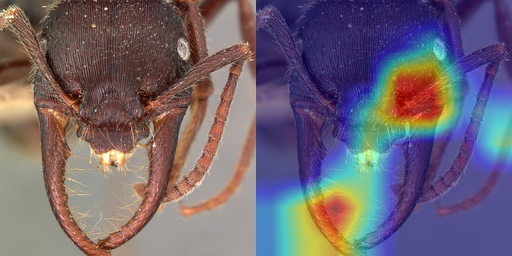
\includegraphics[width=1\linewidth]{thesis_assets/gradcam/incorrect_nonideal/1.png}
        \label{fig:incorrect_nonideal_1}
    \end{subfigure}
    \begin{subfigure}{\subwidth}
        \caption*{Rough texture}
        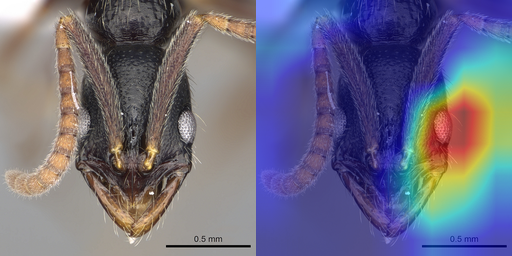
\includegraphics[width=1\linewidth]{thesis_assets/gradcam/incorrect_nonideal/22.png}
        \label{fig:incorrect_nonideal_22}
    \end{subfigure}
    \begin{subfigure}{\subwidth}
        \caption*{Rough texture}
        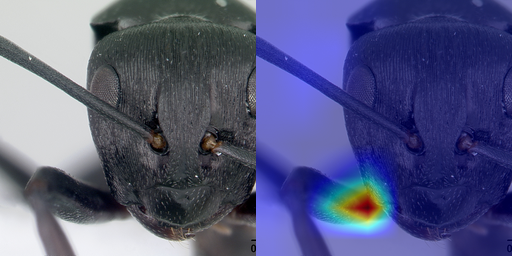
\includegraphics[width=1\linewidth]{thesis_assets/gradcam/incorrect_nonideal/61.png}
        \label{fig:incorrect_nonideal_61}
    \end{subfigure}
    \begin{subfigure}{\subwidth}
        \caption*{Rough texture}
        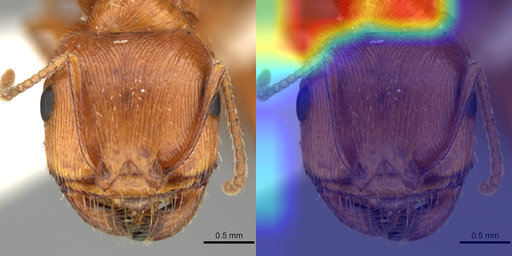
\includegraphics[width=1\linewidth]{thesis_assets/gradcam/incorrect_nonideal/204.png}
        \label{fig:incorrect_nonideal_204}
    \end{subfigure}
    \caption{GradCAM visualization for incorrectly classified images from
        fine-tuned ResNet101. The red sections of the heatmap show which features
        had higher activation for the classication.}
    \label{fig:incorrect_images}
\end{figure}

\newcommand{\segmentedsubwidth}{0.24\textwidth}
\begin{figure}
    \centering
    \begin{subfigure}{\segmentedsubwidth}
        \caption*{Rough texture}
        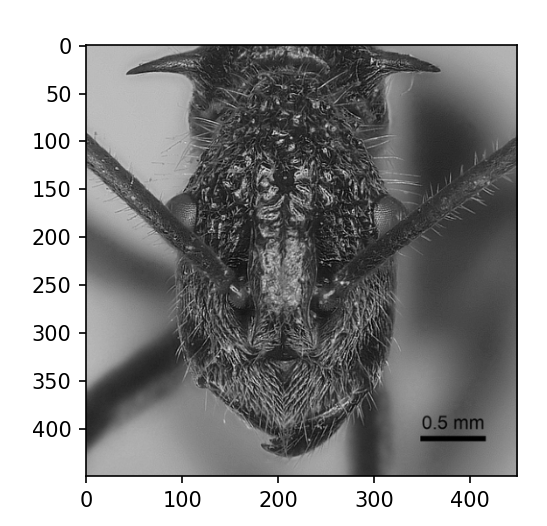
\includegraphics[width=1\linewidth]{figs/r103.png}
    \end{subfigure}
    \begin{subfigure}{\segmentedsubwidth}
        \caption*{Rough texture}
        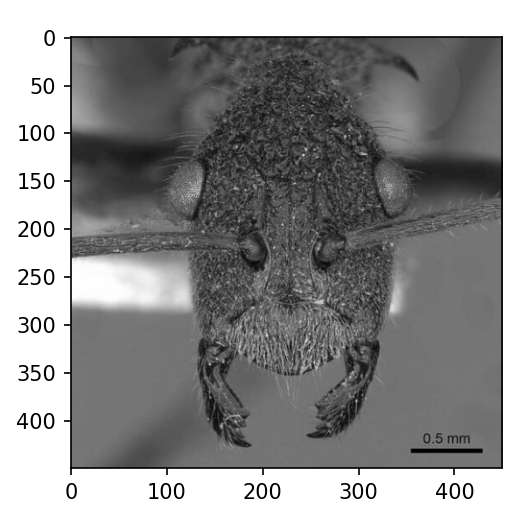
\includegraphics[width=1\linewidth]{figs/r111.png}
    \end{subfigure}
    \begin{subfigure}{\segmentedsubwidth}
        \caption*{Smooth texture}
        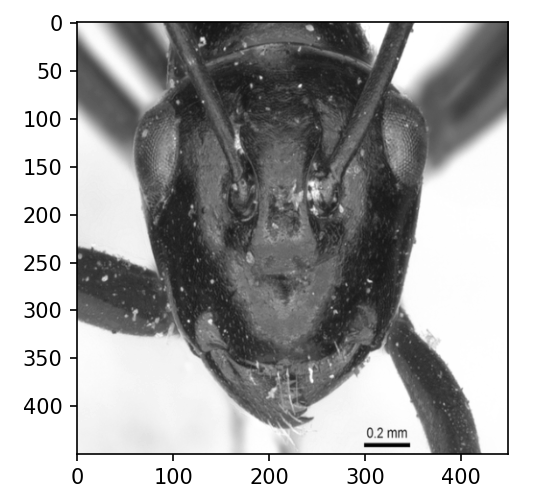
\includegraphics[width=1\linewidth]{figs/s105.png}
    \end{subfigure}
    \begin{subfigure}{\segmentedsubwidth}
        \caption*{Smooth texture}
        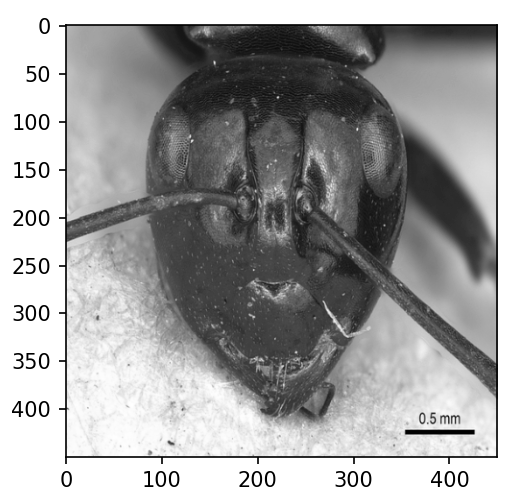
\includegraphics[width=1\linewidth]{figs/s107.png}
    \end{subfigure}

    \begin{subfigure}{\segmentedsubwidth}
        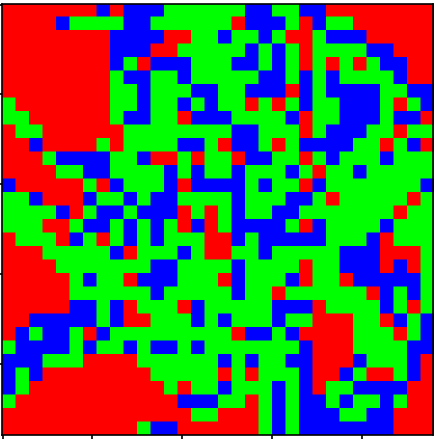
\includegraphics[width=1\linewidth]{figs/15/r103.png}
    \end{subfigure}
    \begin{subfigure}{\segmentedsubwidth}
        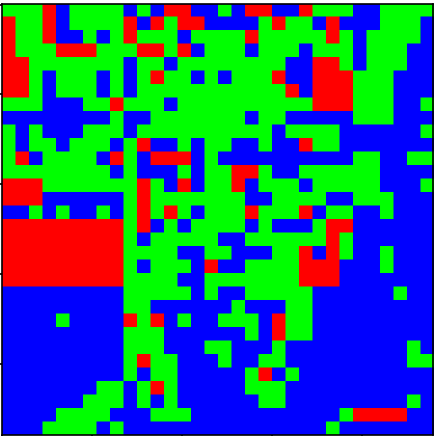
\includegraphics[width=1\linewidth]{figs/15/r111.png}
    \end{subfigure}
    \begin{subfigure}{\segmentedsubwidth}
        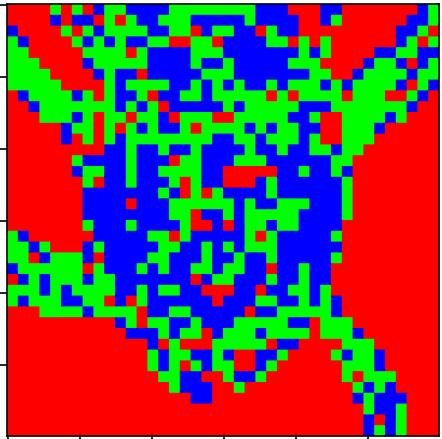
\includegraphics[width=1\linewidth]{figs/15/s105.png}
    \end{subfigure}
    \begin{subfigure}{\segmentedsubwidth}
        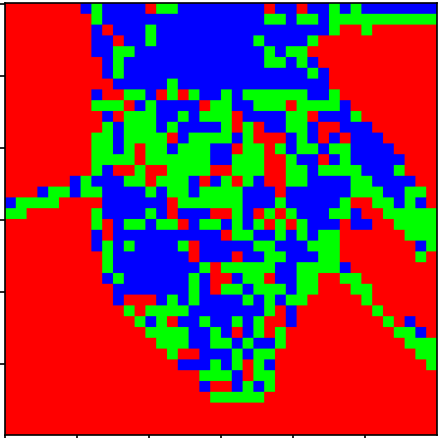
\includegraphics[width=1\linewidth]{figs/15/s107.png}
    \end{subfigure}

    \begin{subfigure}{\segmentedsubwidth}
        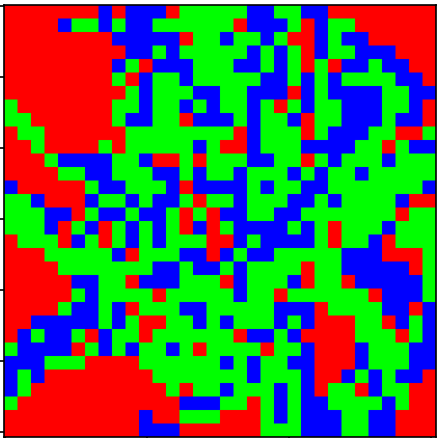
\includegraphics[width=1\linewidth]{figs/19/r103.png}
    \end{subfigure}
    \begin{subfigure}{\segmentedsubwidth}
        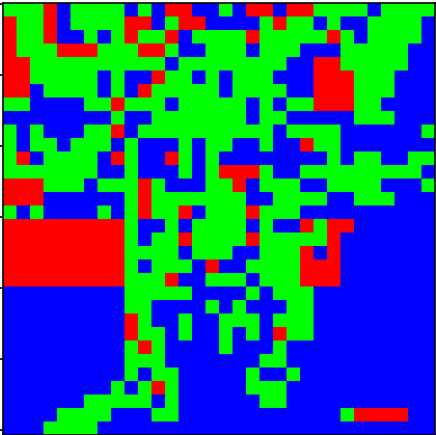
\includegraphics[width=1\linewidth]{figs/19/r111.png}
    \end{subfigure}
    \begin{subfigure}{\segmentedsubwidth}
        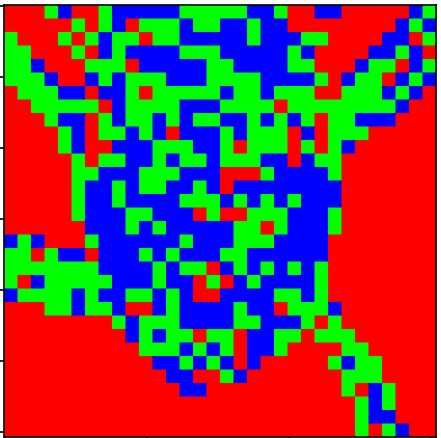
\includegraphics[width=1\linewidth]{figs/19/s105.png}
    \end{subfigure}
    \begin{subfigure}{\segmentedsubwidth}
        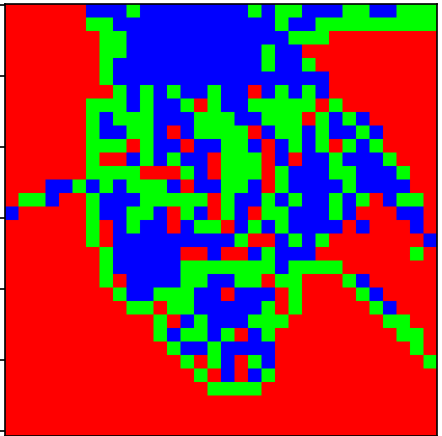
\includegraphics[width=1\linewidth]{figs/19/s107.png}
    \end{subfigure}
    \caption{Raw images are shown with corresponding segmented outputs from
        K-views algorithm. The second row shows the results of using size of 15
        $\times$ 15 patches. The third row shows the results of using size of 19
        $\times$ 19 patches. In the images, the color red represents the
        background class, green represents the smooth class, and the blue
        represent the rough class.}
    \label{fig:kviews_segmented}
\end{figure}

\FloatBarrier Some classified results from the K-views are shown in Figure
\ref{fig:kviews_segmented}. A training set of 550 patches for background, 455
patches for rough, and 493 patches for smooth are used with patch sizes of 15
$\times$ 15 and 19 $\times$ 19. These patches are extracted from two rough and
two smooth images with sizes of 608 $\times$ 608. The K-views algorithm
converges early although we set the maximum number of iterations to be 1000.
These experimental results are preliminary due to the minimal number of source
images used and future work will explore a more expansive approach to the
problem.

\section{Conclusions}
We have shown in this work that a deep learning approach and classical image
texture analysis methods can be used to automatically categorize ants based on
their cuticle texture, therefore supporting research on the evaluation of the
cuticle micro sculpturing function in future work. Our categorization system is
novel in the field of automated insect identification due to the broad number of
species captured by it. A model that is pre-trained on a diverse image task such
as ResNet can be transferred to our domain of texture analysis\footnote{All code
    is publicly available on GitHub \url{https://github.com/ngngardner/cuticulus}}.
However, a deep learning algorithm created specifically for the domain of
texture analysis had an F1 score of 92\% in our experiments. In future work, we
will continue to explore texture classes present in the dataset which are not
captured by the binary class system. We will also investigate application of
texture-based deep maching learning in image texture analysis.

\section*{Conflict of interest}
All authors declare no conflicts of interest in this paper.

\bibliographystyle{AIMS}
\bibliography{main.bib,article.bib}
\end{document}
